%% This is an example first chapter.  You should put chapter/appendix that you
%% write into a separate file, and add a line \include{yourfilename} to
%% main.tex, where `yourfilename.tex' is the name of the chapter/appendix file.
%% You can process specific files by typing their names in at the 
%% \files=
%% prompt when you run the file main.tex through LaTeX.
\chapter{Methodology and Datasets}\label{chap:method}
\section{Tracking by detection approach}
Tracking multiple objects is the task of assigning unique and consistent identifiers to multiple objects in a video series. This article investigates an object tracking technique called "tracking by detection". Tracking through detection is a two-stage process: the object detection algorithm first detects the objects present in the frame; then the detection is done. These objects are then linked to those that have been tracked through a tracking algorithm. Usually, the object detection algorithm and tracking algorithm are completely separate from each other, so they can be analyzed separately.
Object detection is the process of detecting specific categories of objects in an image, examples of these categories are things such as pedestrian or car. The purpose of the object detection algorithm is to locate and classify objects belonging to any popular category. Therefore, for each detected object, the object detection algorithm produces an estimate of the object's location, size, and category. The position and size of the detected object are usually represented by a bounding box, which is a rectangular box surrounding the object. The range of the detected object can also be defined by a segmentation mask, which is a pixel-level mask of the object.
Due to recent advances in the field of image classification, target detection has made considerable progress. This progress is attributed to a breakthrough in how to use CNN for image classification \cite{10.1145/3065386}. The target detection algorithm considered in this paper usually consists of a CNN designed for image classification, and then has an algorithm-specific additional structure around the CNN. CNN is called the backbone of the algorithm, and the algorithm-specific structure is called the meta-architecture. By convention, this paper will identify object detection algorithm through its meta-architecture. CNN-based object detection algorithm can be divided into two different groups: single-stage and two-stage detectors \cite{DBLP:journals/corr/abs-1808-07256}. The two-stage detector first is possible bounding boxes by segmenting the image into regions of interest, and then CNN classifies these regions in the second stage. The single-stage detector is bounding box and class estimates in a single forward pass of the image through the CNN. Traditionally, two-stage detectors have achieved higher accuracy at the expense of speed compared to single-stage detectors. However, the recently introduced loss function Focal loss \cite{DBLP:journals/corr/abs-1708-02002} makes the accuracy of a single-stage detector close to that of a two-stage detector. The trade-off between speed and accuracy is the main design choice, as studied in the paper \cite{DBLP:journals/corr/HuangRSZKFFWSG016}.
The tracking algorithm in the "tracking by detection" framework is responsible for assigning unique identifiers to the tracked objects and establishing object associations between frames. This article focuses on target detection algorithm, and only considers two different tracking algorithm: SORT and DeepSORT SORT stands for simple online and real-time tracking. It is a deliberately simple tracking algorithm that uses a Kalman filter \cite{10.1115/1.3662552} to estimate the future position of an object, and uses the Hungarian method \cite{doi:10.1002/nav.3800020109} for frame-to-frame correlation. Deep SORT is an extension of SORT that incorporates appearance information when performing object association between frames.
\section{Object detection and segmentation algorithms}
\subsection{RCNN model family}
\subsubsection{RCNN}
R-CNN is an abbreviation for regions with CNN features, and is an object detection method introduced by Girschick et al in \cite{DBLP:journals/corr/GirshickDDM13}. The system is a pipeline consisting of three main parts: region proposal, convolutional neural network and a set of support vector machines (SVM).
Figure \ref{fig:rcnnSche} below shows the interaction of the main parts of R-CNN. First, the region proposal method divides the image into regions irrelevant to the category. Each image produces approximately 2000 regions. After segmenting the image, each region is deformed into a fixed size to fit the required input size of the CNN. Next, feed 2000 deformed regions through CNN, and extract feature vectors for each region. Then, the feature vectors are registered by a set of linear SVMs, where each SVM is trained to classify a specific category. Finally, given the class predicted by SVM, ridge regression is used to improve the predicted shape of the bounding box. Given a predicted bounding box coordinate \(p=(p_x,p_y,p_w,p_h)\) (center coordinate, width, height) and its corresponding ground truth box coordinates \(g=(g_x,g_y,g_w,g_h )\), the regressor is configured to learn scale-invariant transformation between two centers and log-scale transformation between widths and heights. All the transformation functions take p as input.
\begin{equation}
	\hat g_x=p_w d_x (p)+p_x
\end{equation}
\begin{equation}
	\hat g_y=p_h d_x (p)+p_y
\end{equation}
\begin{equation}
	\hat g_w=p_w \exp{(d_w(p))}
\end{equation}
\begin{equation}
	\hat g_h=p_h \exp{(d_h(p))}
\end{equation}
\begin{figure}
	\centerline{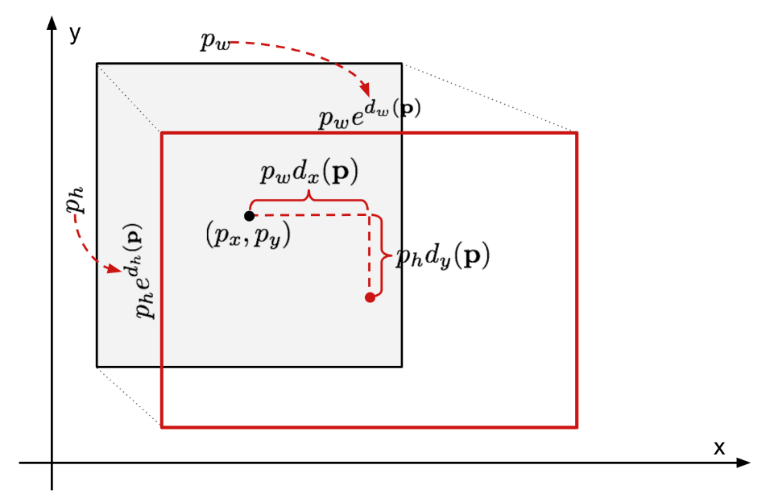
\includegraphics[width=0.5\linewidth]{Figs/rcnnTrans.png}}
	\caption{Illustration of transformation between predicted and ground truth bounding boxes.}
	\label{fig:rcnnTrans}
\end{figure}
An obvious benefit of applying such transformation is that all the bounding box correction functions, \(d_i (p)\) where \( i\in {x,y,w,h}\), can take any value between \([-\infty,+\infty]\). The targets for them to learn are:
\begin{equation}
	t_x=(g_x-p_x )/p_w
\end{equation}
\begin{equation}
	t_y=(g_y-p_y )/p_h
\end{equation}
\begin{equation}
	t_w=\log{(g_w/p_w)} 
\end{equation}
\begin{equation}
	t_h=\log{(g_h/p_h)} 
\end{equation}
A standard regression model can solve the problem by minimizing the SSE loss with regularization:
\begin{equation}
	\mathcal{L}_{reg} = \sum_{i \in (x,y,w,h)}(t_i-d_i(p))^2 + \lambda||w||^2
\end{equation}
The regularization term is critical here and RCNN paper picked the best \(\lambda\) by cross validation. It is also noteworthy that not all the predicted bounding boxes have corresponding ground truth boxes. For example, if there is no overlap, it does not make sense to run bbox regression. Here, only a predicted box with a nearby ground truth box with at least 0.6 IoU is kept for training the bbox regression model.
\\After scoring all regions, non-maximum suppression will be applied to remove prediction bounding boxes that overlap with predictions with higher scores. R-CNN is not limited to any specific segmentation method or specific CNN architecture. In \cite{DBLP:journals/corr/GirshickDDM13}, a segmentation method called selective search \cite{6126456} is used, and the results of using the CNN system structure introduced in \cite{10.1145/3065386} and \cite{Simonyan2015VeryDC} are demonstrated.
\\The author of R-CNN also shows that supervised pre-training for similar problems is an effective way to initialize CNN weights. In \cite{DBLP:journals/corr/GirshickDDM13}, pre-trained CNN is used to classify the data from ILSVRC2013 to obtain the initial weight of CNN \cite{DBLP:journals/corr/RussakovskyDSKSMHKKBBF14}. Then, by training it on the Pascal VOC 2012 dataset, fine-tune the CNN to perform object detection, which is an object detection dataset. This is a form of transfer learning, which has proven to be an effective method when adapting CNN to a domain with sparse training data \cite{DBLP:journals/corr/abs-1808-01974}.
\begin{figure}
	\centerline{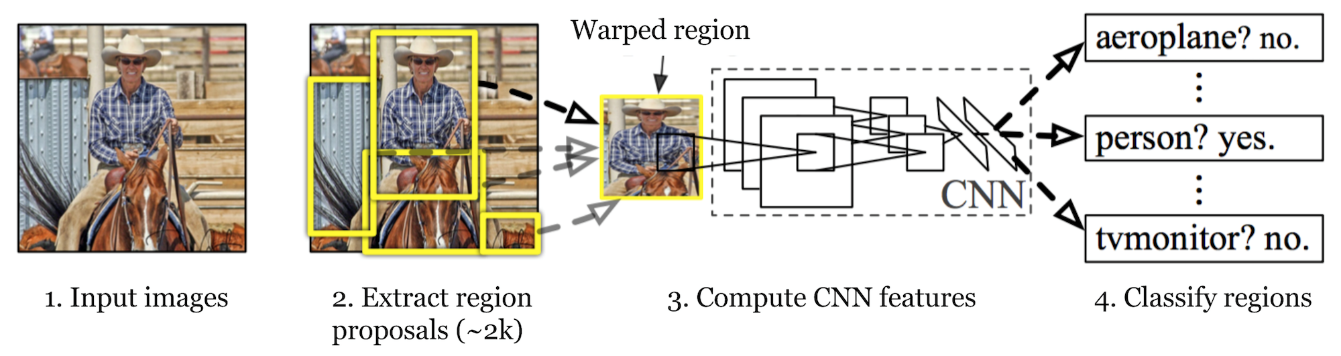
\includegraphics[width=1\linewidth]{Figs/rcnnSche.png}}
	\caption{Schematic of the R-CNN pipeline.}
	\label{fig:rcnnSche}
\end{figure}
\subsubsection{FastRCNN}
The main disadvantage of the R-CNN method is its slow speed. This is mainly because each regional proposal is passed through CNN separately, which is very time-consuming. In order to improve the speed, Girshick introduced a target detection method called Fast R-CNN in \cite{DBLP:journals/corr/Girshick15}. Fast R-CNN can improve the speed of object detection, mainly by passing the image forward through CNN only once, rather than once for each region performed by R-CNN. As in R-CNN, the region proposal method first divides the image into category-independent regions, creating a region of interest (RoI). Then, the entire image is processed by a CNN, which does a convolutional feature map of the image. Next, for each regional proposal, the RoI pool layer using spatial pyramid pool \cite{DBLP:journals/corr/HeZR014} is applied to the feature map. This will convert each RoI into a fixed-size vector. Then, the feature vectors are processed by fully connected layers, which are divided into two different output layers. One of the output layers is the softmax layer, which estimates probability estimates for object classes. The other layer is the bounding box regressor, which outputs a refined estimate of the bounding box for each object class. Figure \ref{fig:fastArc} shows how an image is processed by Fast R-CNN.
\begin{figure}
	\centerline{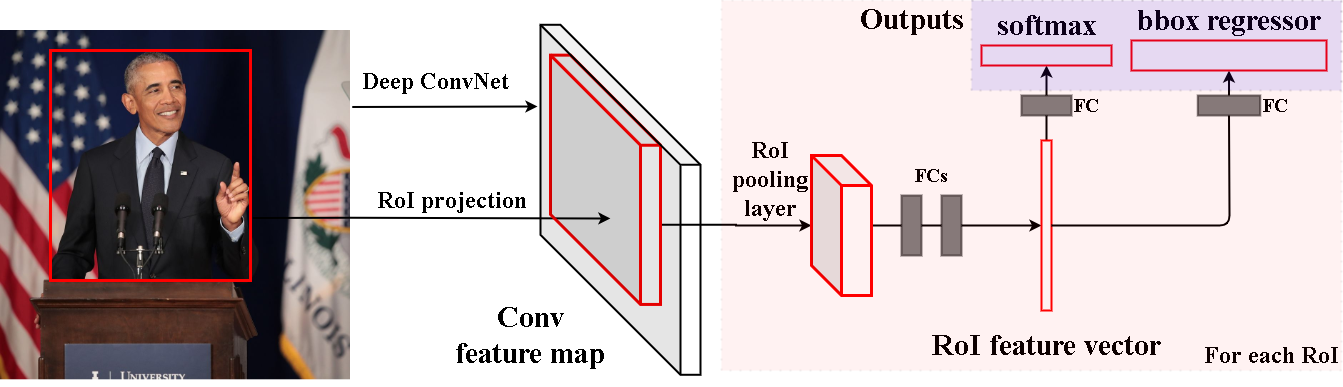
\includegraphics[width=0.5\linewidth]{Figs/fastArc.png}}
	\caption{The architecture of Fast RCNN.}
	\label{fig:fastArc}
\end{figure}
The model is optimized for a loss combining two tasks (classification + localization):
\begin{table}[]
	\begin{tabular}{|l|l|}
		\hline
		Symbol                                          & Explanation                                                                                                                                                                                                  \\ \hline
		u                                              & \begin{tabular}[c]{@{}l@{}}True class label, \(u \in 0,1,…,K\); by convention, the catch-all background\\ class has \(u=0\)\end{tabular}                                                                    \\ \hline
		p                                              & \begin{tabular}[c]{@{}l@{}}Discrete probability distribution (per RoI) over K + 1 classes:\\ \(p=(p_0,…,p_K)\), computed by a softmax over the K + 1 outputs of a fully\\ connected layer.\end{tabular} \\ \hline
		v                                              & True bounding box \(v=(v_x, v_y, v_w, v_h)\).                                                                                     \\ \hline
		\begin{tabular}[c]{@{}l@{}} \(t^u\)\end{tabular} & Predicted bounding box correction, \(t^u=(t^u_x, t^u_y, t^u_w, t^u_h)\).                                                                                                                                                                         \\ \hline
	\end{tabular}
	\caption{Some definitions for calculating FastRCNN losses.}
\end{table}
The loss function sums up the cost of classification and bounding box prediction: \(\mathcal{L} = \mathcal{L}_{cls} + \mathcal{L}_{box}\). For “background” RoI, \(\mathcal{L}_{box}\) is ignored by the indicator function
\(f [u \geq 1]\), defined as in equation \ref{eq:mathbb}.
\begin{equation}
	\label{eq:mathbb}
f [u >= 1] = \begin{cases}
	1  & \text{if } u \geq 1\\
	0  & \text{otherwise}
\end{cases}
\end{equation}
The overall loss function is:
\begin{equation}
	\mathcal{L}(p, u, t^u, v) = \mathcal{L}_{cls} (p, u) + f [u \geq 1] \mathcal{L}_{box}(t^u, v)
\end{equation}\begin{equation}
	\mathcal{L}_{cls}(p, u) = -\log p_u
\end{equation}
\begin{equation}
	\mathcal{L}_{box}(t^u, v) = \sum_{i \in \{x, y, w, h\}} L_1^{smooth} (t^u_i - v_i)
\end{equation}
The bounding box loss \(\mathcal{L}_{box}\) should measure the difference between \(t^u_i\) and \(v_i\) using a robust loss function. The smooth L1 loss is adopted here and it is claimed to be less sensitive to outliers.
\subsubsection{FasterRCNN}
Fast R-CNN passing the speed of object detection by passing the image forward through the CNN only once, instead of forward passing through each region of interest in the image. For Fast R-CNN, the bottleneck lies in the image segmentation method usually implemented on the CPU. In order to solve this problem, Ren et al. A method called Faster R-CNN is proposed in \cite{DBLP:journals/corr/RenHG015}. Faster R-CNN eliminates the need for CPU computing by introducing the idea of a Region Proposal Networks (RPNs). The region proposal network to region proposed by sliding a small network on the convolutional feature map. At each location, the small network takes a window of the convolution feature map and converts it into a feature vector. This feature vector is then input into two different fully connected layers, one layer performs bounding box regression, and the other layer is a classification layer that predicts objective scores. The objectivity score is a prediction of the probability that the predicted bounding box contains only one object compared to the background.
\\For each position, RPN makes several predictions relative to a fixed number of reference frames, which are called anchors. You can anchor as a suggested border for each sliding window position. In \cite{DBLP:journals/corr/RenHG015}, anchors are created in 3 ratios and 3 different aspect ratios, and each position provides a total of 9 different anchors. This means that RPN has 9 bounding boxes at each sliding window position, and each anchor point has one bounding box.
\begin{figure}
	\centerline{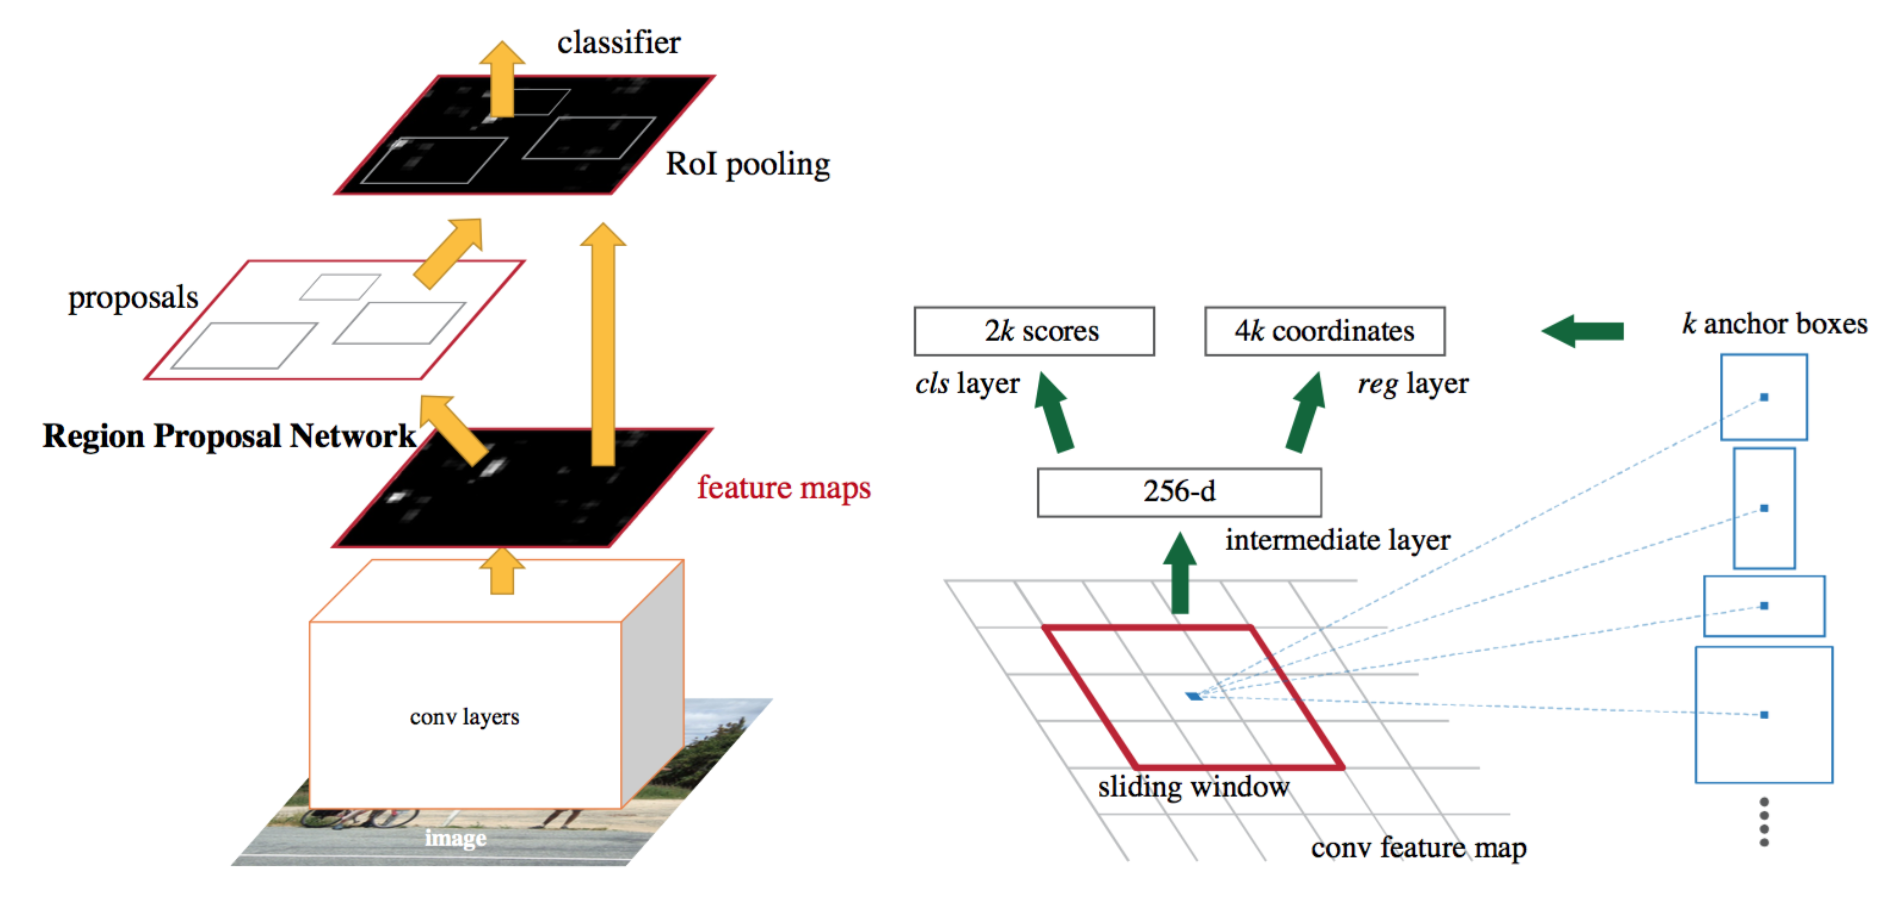
\includegraphics[width=0.5\linewidth]{Figs/faster.png}}
	\caption{An illustration of Faster RCNN model.}
	\label{fig:faster}
\end{figure}
\\The regions generated by RPN are then used as region suggestions in fast RCNN. By using RPN, Faster R-CNN eliminates the time-consuming image segmentation required in Fast R-CNN. By using a single CNN for RPN and fast R-CNN, the speed is further increased. This also means that the Faster R-CNN can be trained end-to-end by first training the RPN to propose a region, and then using the region proposal to train the Fast R-CNN.
\\Faster R-CNN is optimized for a multi-task loss function, similar to fast R-CNN.
\begin{table}[]
	\label{tab:noteFaster}
	\begin{tabular}{|l|l|}
		\hline
		Symbol & Explanation                                                                                                                                                           \\ \hline
		\(p_i\)      & Predicted probability of anchor i being an object.                                                                                                                    \\ \hline
		\(p_i^*\)      & Ground truth label (binary) of whether anchor i is an object.                                                                                                         \\ \hline
		\(t_i\)      & Predicted four parameterized coordinates.                                                                                                                             \\ \hline
		\(t_i^*\)      & Ground truth coordinates.                                                                                                                                             \\ \hline
		\(N_{cls}\)      & Normalization term, set to be mini-batch size ($\sim$256) in the paper.                                                                                               \\ \hline
		\(N_{box}\)      & \begin{tabular}[c]{@{}l@{}}Normalization term, set to the number of anchor locations ($\sim$2400) in\\ the paper.\end{tabular}                                        \\ \hline
		$\lambda$      & \begin{tabular}[c]{@{}l@{}}A balancing parameter, set to be $\sim$10 in the paper (so that both \(\mathcal{L}_{cls}\) and\\ \(\mathcal{L}_{box}\) terms are roughly equally weighted).\end{tabular} \\ \hline		
	\end{tabular}
\caption{Some definitions for calculating FasterRCNN losses.}
\end{table}
With notation in Table \ref{tab:noteFaster} the multi-task loss function combines the losses of classification and bounding box regression:
\begin{equation}
	\mathcal{L}_{reg} = \mathcal{L}_{cls} + \mathcal{L}_{box}
\end{equation}
\begin{equation}
	\mathcal{L}(\{p_i\}, \{t_i\})= \frac{1}{N_{cls}} \sum_i \mathcal{L}_{cls} (p_i, p^*_i) + \frac{\lambda}{N_{box}} \sum_i p^*_i \cdot L_1^{smooth}(t_i - t^*_i) \\
\end{equation}
where \(\mathcal{L}_{cls}\) is the log loss function over two classes, as we can easily translate a multi-class classification into a binary classification by predicting a sample being a target object versus not. \(L_1^{smooth}\) is the smooth L1 loss.
\begin{equation}
	\mathcal{L}_{cls} (p_i, p^*_i) = - p^*_i \log p_i - (1 - p^*_i) \log (1 - p_i)
\end{equation}
\subsubsection{MaskRCNN}
The mask R-CNN is an extension of Faster R-CNN proposed by He et al in \cite{DBLP:journals/corr/HeGDG17}. In addition to object detection, Mask R-CNN can also perform object instance segmentation. Segmentation is achieved by adding a third branch to Faster R-CNN, which outputs an object mask for each detected object. In order to improve the segmentation, a method called RoIAlign is introduced to extract more accurate feature maps for each RoI. RoIAlign uses bilinear interpolation instead of quantizing the feature map to calculate the exact value of the feature map.
\begin{figure}
	\centerline{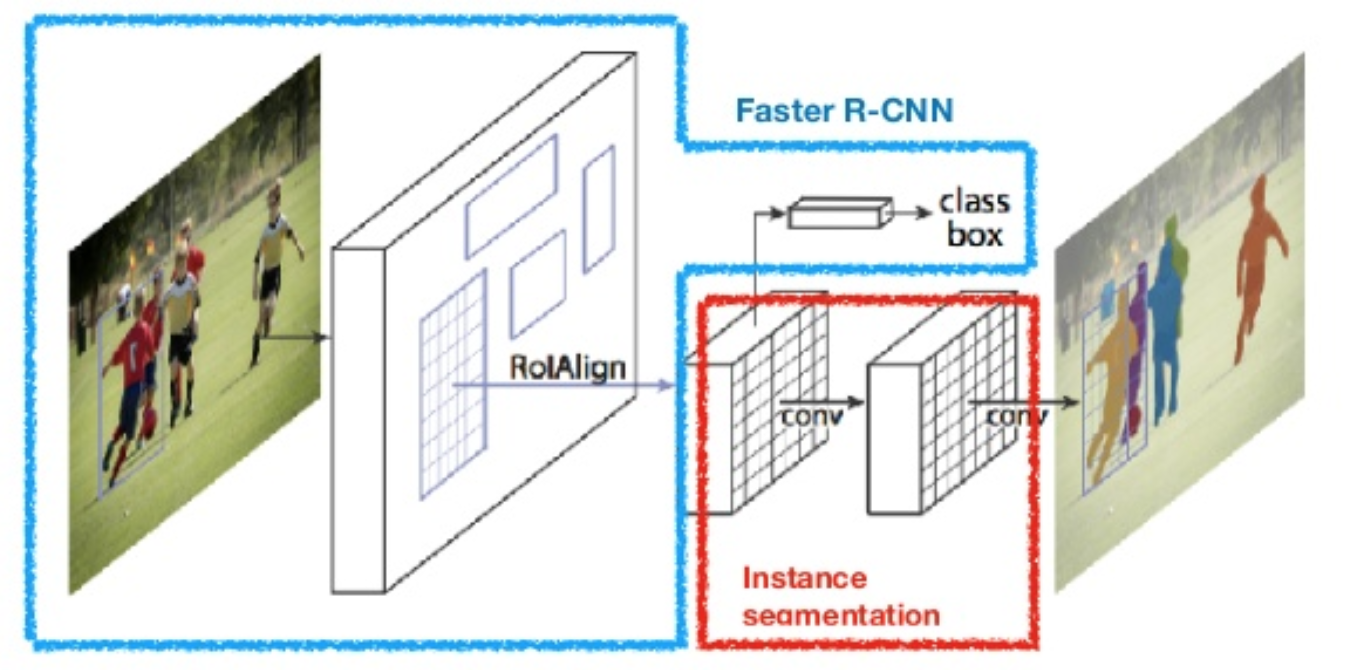
\includegraphics[width=0.5\linewidth]{Figs/maskrcnn.png}}
	\caption{The Mask RCNN framework for instance segmentation.}
	\label{fig:maskrcnn}
\end{figure}
The author of \cite{DBLP:journals/corr/HeGDG17} found that Mask R-CNN has a higher average accuracy than Faster R-CNN in target detection. It turns out that this is partly due to the use of RoIAlign and partly due to the multi-task loss used to train Mask R-CNN. Mask R-CNN has a multi-task loss function, which can simultaneously consider classification, bounding box regression and object segmentation.
The multi-task loss function of Mask R-CNN combines the loss of classification, localization and segmentation mask: 
\begin{equation}
	\mathcal{L} = \mathcal{L}_{cls} + \mathcal{L}_{box}+ \mathcal{L}_{mask}
\end{equation}
where \(\mathcal{L}_{cls}\) and \(\mathcal{L}_{box}\) are same as in Faster R-CNN.
The mask branch generates a mask of dimension m x m for each RoI and each class; K classes in total. Thus, the total output is of size \(K \cdot m^2\). Because the model is trying to learn a mask for each class, there is no competition among classes for generating masks. \(\mathcal{L}_{mask}\) is defined as the average binary cross-entropy loss, only including k-th mask if the region is associated with the ground truth class k.
\begin{equation}
	\mathcal{L}_{mask} = - \frac{1}{m^2} \sum_{1 \leq i, j \leq m} \big[ y_{ij} \log \hat{y}^k_{ij} + (1-y_{ij}) \log (1- \hat{y}^k_{ij}) \big]\
\end{equation}
where \(y_{ij}\) is the label of a cell (i, j) in the true mask for the region of size m x m; \(\hat{y}_{ij}^k\) is the predicted value of the same cell in the mask learned for ground-truth class k.
\subsection{YOLO model family}
\subsubsection{YOLO}
In \cite{DBLP:journals/corr/RedmonDGF15}, a novel object detection method is introduced, called YOLO, which means "You Only Look Once". Unlike R-CNN and its successors, YOLO does not use any region proposal method, but uses a single CNN to predict bounding boxes and classes. 
\\In YOLO, the input image is first divided into S × S grids. Then, each grid unit is responsible for predicting the bounding box B and the confidence score of each bounding box. The formula for calculating the confidence score is \(Pr(Object)*IoU_{pred}^{gt}\), where Pr(Object) is the predicted probability that the box contains an object, and \(IoU_{pred}^{gt}\) is the estimated intersection over union (IoU) between the predicted box and the ground truth box. For each grid unit, the probability of object categories C can also be predicted, and these probabilities are conditioned on the unit containing the object. The predicted box and class probabilities are then combined into a single score for each class and box. 
\\Equation \ref{eq:yolo} comes from the introduction by YOLO in \cite{DBLP:journals/corr/RedmonDGF15}, which shows how class prediction and box prediction are combined. As shown in the original paper, \(Pr(Class_i)\) is used as a simplified representation of \(Pr(Class_i|Object)\).
\begin{equation}
	\label{eq:yolo}
	Pr(Class_i|Object)*Pr(Object)*IoU^{gt}_{pred} = Pr(Class_i)*IoU^{gt}_{pred}
\end{equation}
This score not only explains the probability that the box contains class \(i\), \(Pr(Class_i)\), but also how to estimate the predicted box to fit the ground truth box \(Pr(Object)*IoU_{pred}^{gt}\). 
%Figure \ref{fig:yoloworkflow} shows how to split the image into a grid, and how the cell with the dot as the center predicts different bounding boxes. The predicted bounding box is then combined with the class probabilities also obtained from the image grid to produce the final object detection.
%\begin{figure}
%	\centerline{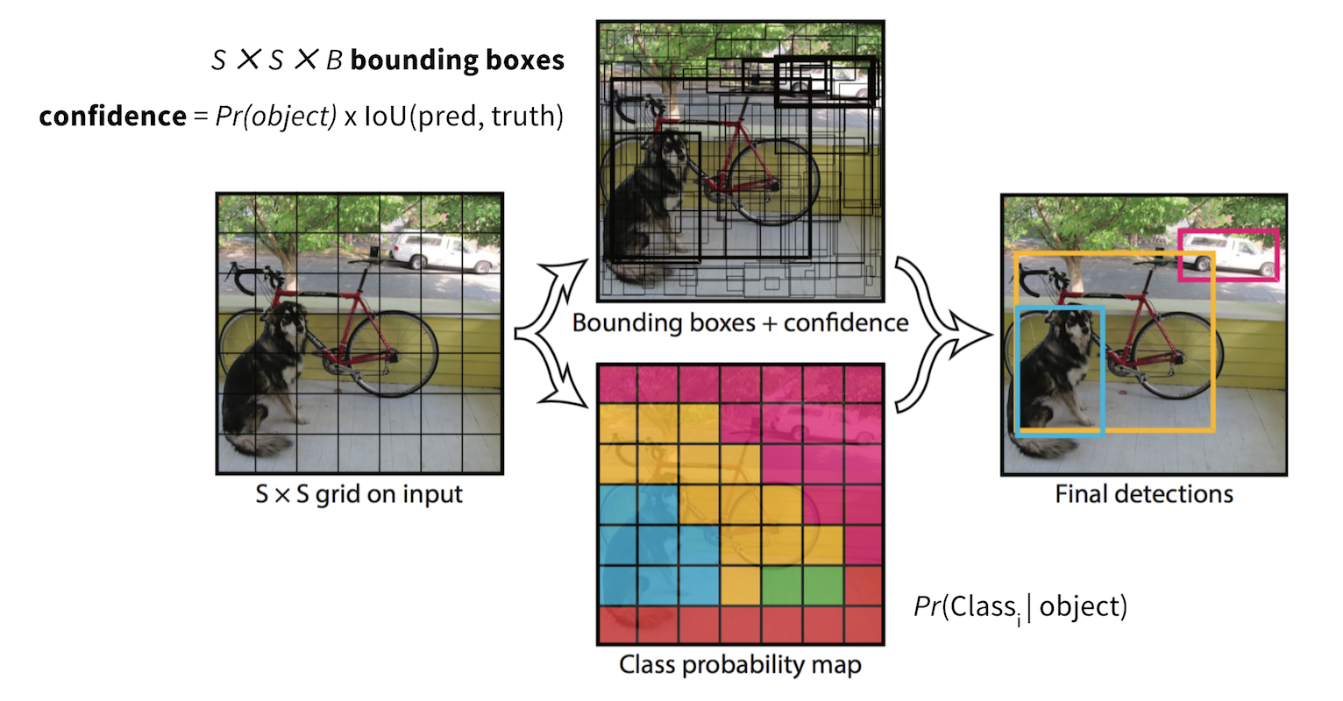
\includegraphics[width=1\linewidth]{Figs/yoloworkflow.png}}
%	\caption{The workflow of YOLO model.}
%	\label{fig:yoloworkflow}
%\end{figure}
The base model \ref{fig:yolo-network} is similar to GoogLeNet with inception module replaced by 1x1 and 3x3 conv layers. The final prediction of shape S×S×(5B+K) is produced by two fully connected layers over the whole conv feature map.
\begin{figure}
	\centerline{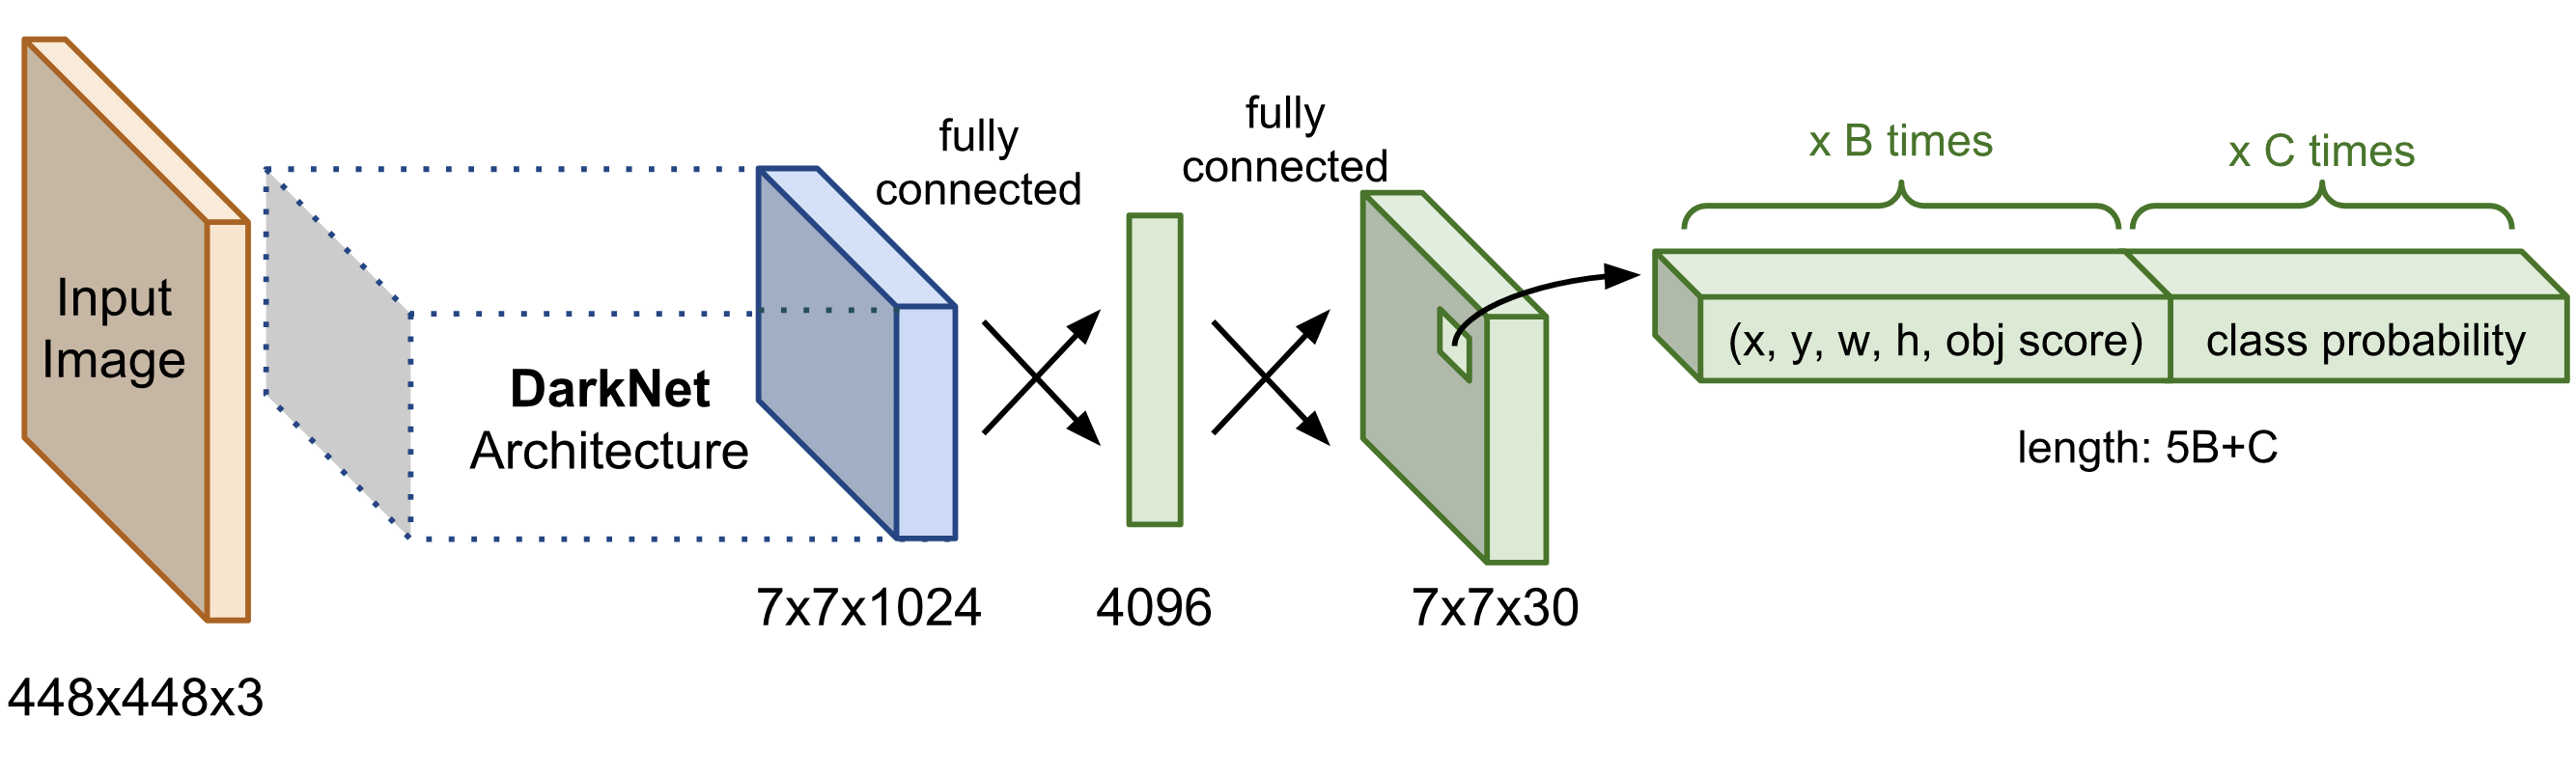
\includegraphics[width=1\linewidth]{Figs/yolo-network.png}}
	\caption{The network architecture of YOLO.}
	\label{fig:yolo-network}
\end{figure}
\subsubsection{YOLOv2}
In order to improve YOLO, Redmon et al. proposed a method called YOLOv2 in \cite{DBLP:journals/corr/RedmonF16}. YOLOv2 is a modified version of YOLO, designed to improve speed and accuracy.
Similar to Faster R-CNN, YOLOv2 uses anchor points when predicting the bounding box. For each grid unit, YOLOv2 generates a bounding box by predicting the offset of 5 anchor points. It is now also possible to predict the class for each anchor point instead of each grid unit, and also provide an objective score for each anchor point. As in YOLO, the class is predicted under the condition that the object \(Pr(Class_i|Object)\) exists. Objectivity is calculated as the estimated IoU between the predicted box and the estimated ground truth box \(IoU_{pred}^{gt}\). YOLOv2 also uses a new method to determine the anchor point size. YOLOv2 is different from manually selecting anchor points in Faster R-CNN, but uses k-means clustering on the training data to generate anchor points that are more suitable for the data.
In order to increase speed, a CNN architecture called Darknet-19 is introduced in YOLOv2. Darknet-19 is able to achieve higher image classification accuracy than both the widely used VGG-16 [33] and the custom network previously used in YOLO [40]. It manages to do this while only using 5.58 * 109 floating point operations per forward pass, compared to 30.69 * 109 operations in VGG-16 and 8.52 * 109 operations in the network previously used in YOLO.
\subsubsection{YOLOv3}
YOLOv3 includes a further improvement of YOLOv2 proposed by Redmon et al in \cite{DBLP:journals/corr/abs-1804-02767}. Similar to the feature pyramid network (FPN) described in \cite{DBLP:journals/corr/LinDGHHB16}, in YOLOv3, the box will be predicted at 3 different scales. This YOLOv3's ability to detect small objects, which was struggling with earlier versions of YOLO.
Inspired by the residual network proposed in \cite{DBLP:journals/corr/HeZRS15}, Darknet-19 was extended to include a residual layer. This new CNN architecture is called Darknet-53 because it has a total of 53 convolutional layers. Compared with Darknet-19, Darknet-53 has higher accuracy but slower speed.
\vspace{-1.6cm}
\subsubsection{YOLOv4}
So far, YOLOv4 is the latest and most advanced iteration \cite{bochkovskiy2020yolov4}. It has the fastest running speed and can be used for optimization of production systems and parallel computing. Some of the new technologies adopted in YOLOv4 are: (1) weighted residual connection, (2) cross-stage-partial connection, (3) cross mini-batch processing, (4) normalization (CmBN), (5) self-confrontation training, (6) Mish-activation, etc. In order to obtain higher precision values, YOLOv4 uses Dense Block, which is a deeper and more complex network. Similarly, the backbone of its function extractor uses CSPDarknet-53, which deploys CSSP connection with Darkenet-53 of the early YOLOv3. In addition to CSPDarknet-53, YOLOv4's architecture also includes SPP add-on modules, PANet path aggregation neck and YOLOv3 anchor-based head. SPP blocks are stacked on CSPDarknet53 to increase the receiving field that can discretize the most significant context features and ensure that its network operation speed will not decrease. Similarly, PANet is used to aggregate parameters from multiple backbone levels, instead of the FPN used in YOLOv3.
\section{Object tracking algorithms}
\subsection{SORT}
SORT is a tracking algorithm introduced by Bewley et al in \cite{DBLP:journals/corr/BewleyGORU16}. SORT is designed to perform multi-object tracking in a tracking-by-detection system. In order to achieve real-time processing, SORT is deliberately kept simple to avoid performing complex and time-consuming tasks. In order to make up for its lack of complexity, SORT uses CNN-based object detectors instead of relying on more accurate object detection. 
For each new frame, SORT first propagates objects that are already tracked into the current frame. The new positions of these already tracked objects are predicted using a Kalman filter \cite{10.1115/1.3662552} with a linear constant velocity model. Next, an object detection algorithm detects objects present in the current frame. These detected objects are then compared to already tracked objects and a cost-matrix is created. This cost-matrix is calculated as the IoU between each detection and each of the already tracked objects. Detections are then assigned to already tracked objects using the Hungarian method \cite{doi:10.1002/nav.3800020109}. When an object is detected in several consecutive frames and does not overlap with any tracked object, a new trajectory is created. To further explain this point, the object model is represented by equation \ref{eq:kal}, where u, v, s, and r represent the horizontal pixel position, vertical pixel position, area, and aspect ratio of the target object, respectively.
\begin{equation}
	\label{eq:kal}
	X=[u, v, s, r, \dot{u}, \dot{v}, \dot{s}]
\end{equation}
As long as the detection is linked to the target object, the detected bounding box is used to inform the target state, and the Kalman filter is used to solve the level and velocity values. This helps to identify the target's identity in consecutive frames and helps tracking.
\subsection{DeepSORT}
DeepSORT is built to reduce the number of identity switches and integrate appearance information into the tracking process proposed in SORT. Similar to SORT, DeepSORT uses Kalman filter to process state estimation. The difference between DeepSORT and SORT is that it utilizes other technologies when assigning detection to the tracked object.
The first improvement of DeepSORT is the deep appearance descriptor.  To obtain the appearance information of detections and tracks, an appearance descriptor is used to extract features from detection images and track images from previous frames. The appearance descriptor is a CNN trained on large-scale person re-identification dataset. It is able to extract features in a way that features from the same identity are close together and features from different identities are far away from each other in the feature space. The overview of the network architecture of the re-identification model used in DeepSORT framework is shown Table \ref{tab:desarchitecture}.
This thesis customizes the CNN on a custom egocentric hand re-identification dataset, Micand32S. Detail training process is explained in chapter 3, sub-section 3.2.2. Appearance descriptors are computed by forwarding each bounding box through a CNN that has been pretrained on a person re-identification dataset. The appearance descriptor of each new detection is then compared to the appearance descriptors of already tracked objects by calculating the cosine distance between descriptors. Tracked objects and their appearance descriptors are also saved for 30 frames after they are lost so that Deep SORT has the ability to resume tracking identities that have been lost for a number of frames. Using appearance descriptors in this way gives DeepSORT the ability to find a previously tracked object even if it has been occluded for a number of frames.
\begin{table}[]
	\label{tab:desarchitecture}
	\begin{tabular}{|l|l|l|}
		\hline
		Name                       & Patch Size/Stride & Output Size \\ \hline
		Conv1                      & 3x3/1             & 32x128x64   \\ \hline
		Conv2                      & 3x3x1             & 32x128x64   \\ \hline
		Max Pool 3                 & 3x3/2             & 32x64x32    \\ \hline
		Residual 4                 & 3x3/1             & 32x64x32    \\ \hline
		Residual 5                 & 3x3/1             & 32x64x32    \\ \hline
		Residual 6                 & 3x3/2             & 64x32x16    \\ \hline
		Residual 8                 & 3x3/2             & 128x16x8    \\ \hline
		Residual 9                 & 3x3/1             & 128x16x8    \\ \hline
		Dense 10                   &                   & 128         \\ \hline
		Batch and \(L_2\) normalization &                   & 128         \\ \hline
	\end{tabular}
	\caption{Overview of the CNN architecture \cite{DBLP:journals/corr/WojkeBP17}. The final batch and L2 normalization projects onto the unit hyper-sphere.}
\end{table}
The second improvement of DeepSORT is the data association. With the estimated position of the existing tracks and the appearance descriptor, we can now associate new detection results to the existing tracks in each coming frame. A detection confidence threshold td is used to filter out all the detections with confidence lower than the threshold. New detections have to pass this threshold to be candidates of data association. The Deep SORT algorithm uses a cost matrix to represent the spatial and appearance similarities between each new detections and existing tracks. It is integrated by two distance values. The first distance is shown in equation \ref{eq:mahalanobis} representing the spatial information:
\begin{equation}
	\label{eq:mahalanobis}
	d^{(1)}(i,j)=(d_j-y_i)^TS^-1_i(d_j-y_i)
\end{equation}
where \((y_i, S_i)\) are the projection of the i-th track in measurement space and \(d_j\) is the j-th new detection. This is the Mahalanobis distance \cite{hastie2009elements} between j-th new detection and estimated position of i-th. The Mahalanobis distance measures how the position of a new detection differs from the positions of already tracked objects in terms of standard deviations from the mean of the tracked objects. This metric allows DeepSORT to avoid assigning a new detection to an already existing track where the frame-to-frame motion would be unreasonable. The second distance is show in equation \ref{eq:appearance} representing the appearance information.
\begin{equation}
	\label{eq:appearance}
	d^{(2)}(i,j)=min(1-r_j^Tr_k^{(i)}|r_k^{(i)}\in R_i))
\end{equation}
where r is the appearance descriptor and Ri are the appearances of the last 100 object associated with the i-th track. Each distance is accompanied with a gate function \(b_{i,j}^1\)and \(b_{i,j}^2\) which are equal to 1 if the distance is smaller than pre-defined threshold and 0 otherwise. The integrated cost matrix is show in equation \ref{eq:integrated}:
\begin{equation}
	\label{eq:integrated}
	c_{i,j} = \lambda d^{(1)}(i,j) + (1-\lambda)d^{(2)}(i,j)
\end{equation}
With a gate matrix \(b_{i,j}\) which equals to 1 only when both spatial and appearance gate function are equal to 1 and otherwise 0, indicating whether (i, j) is a valid match for both spatial and appearance. In each new frame, the new detections are associated with existing tracks using this cost matrix and gate matrix.
Track handling is processed as follow: every time a new detection is successfully associated with an existing track, the detection is added to the track and the unassociated age of the track is zero. When new detections fail to associate with existing tracks in frame f, the new detections are initialized as Tentative tracks. The original Deep SORT algorithm checks that the Tentative tracks are associated with new detections in each of the  \((f+1), (f+2), ... (f+t_{tentative})\) frames. If successfully associated, the track is updated as Confirmed track. Otherwise, the Tentative track is deleted immediately. As for the existing tracks that fail to associate with new detections in each frame, their unassociated ages will increase by one. If the unassociated age exceeds the max age threshold, the track will also be deleted.
\section{Egocentric vision datasets}\label{sec:datasets}
\subsection{GTEA family datatsets}
Georgia Tech Egocentric Activity Datasets (GTEA) \cite{5995444} contains 7 types of daily activities, each performed by 4 different subjects. The camera is mounted on a cap worn by the subject. 
GTEA Gaze \cite{fathigaze} dataset is collected using Tobii eye-tracking glasses. It consists of 17 sequences, performed by 14 different subjects. GTEA Gaze+ \cite{7298625} is collected by using SMI eye-tracking glasses at Georgia Tech's AwareHome. This dataset consists of 7 meal-preparation activities, performed by 26 subjects. Subjects perform the activities based on the given recipes. Activities are: American Breakfast, Pizza, Snack, Greek Salad, Pasta Salad, Turkey Sandwich and Cheese Burger. SMI glasses record a HD video of subject’s activities at 24 frames per second. They also record subject's gaze at 30 fps. For each activity, ELAN is used to annotate its actions. An activity is a meal-preparation task such as making pizza, and an action is a short temporal segment such as putting sauce on the pizza crust, dicing the green peppers, washing the mushrooms. The authors have completed more than half of the annotations. The current version contains 37 videos with gaze tracking and action annotations. Audio files are also available on request.
%\begin{figure}
%	\centerline{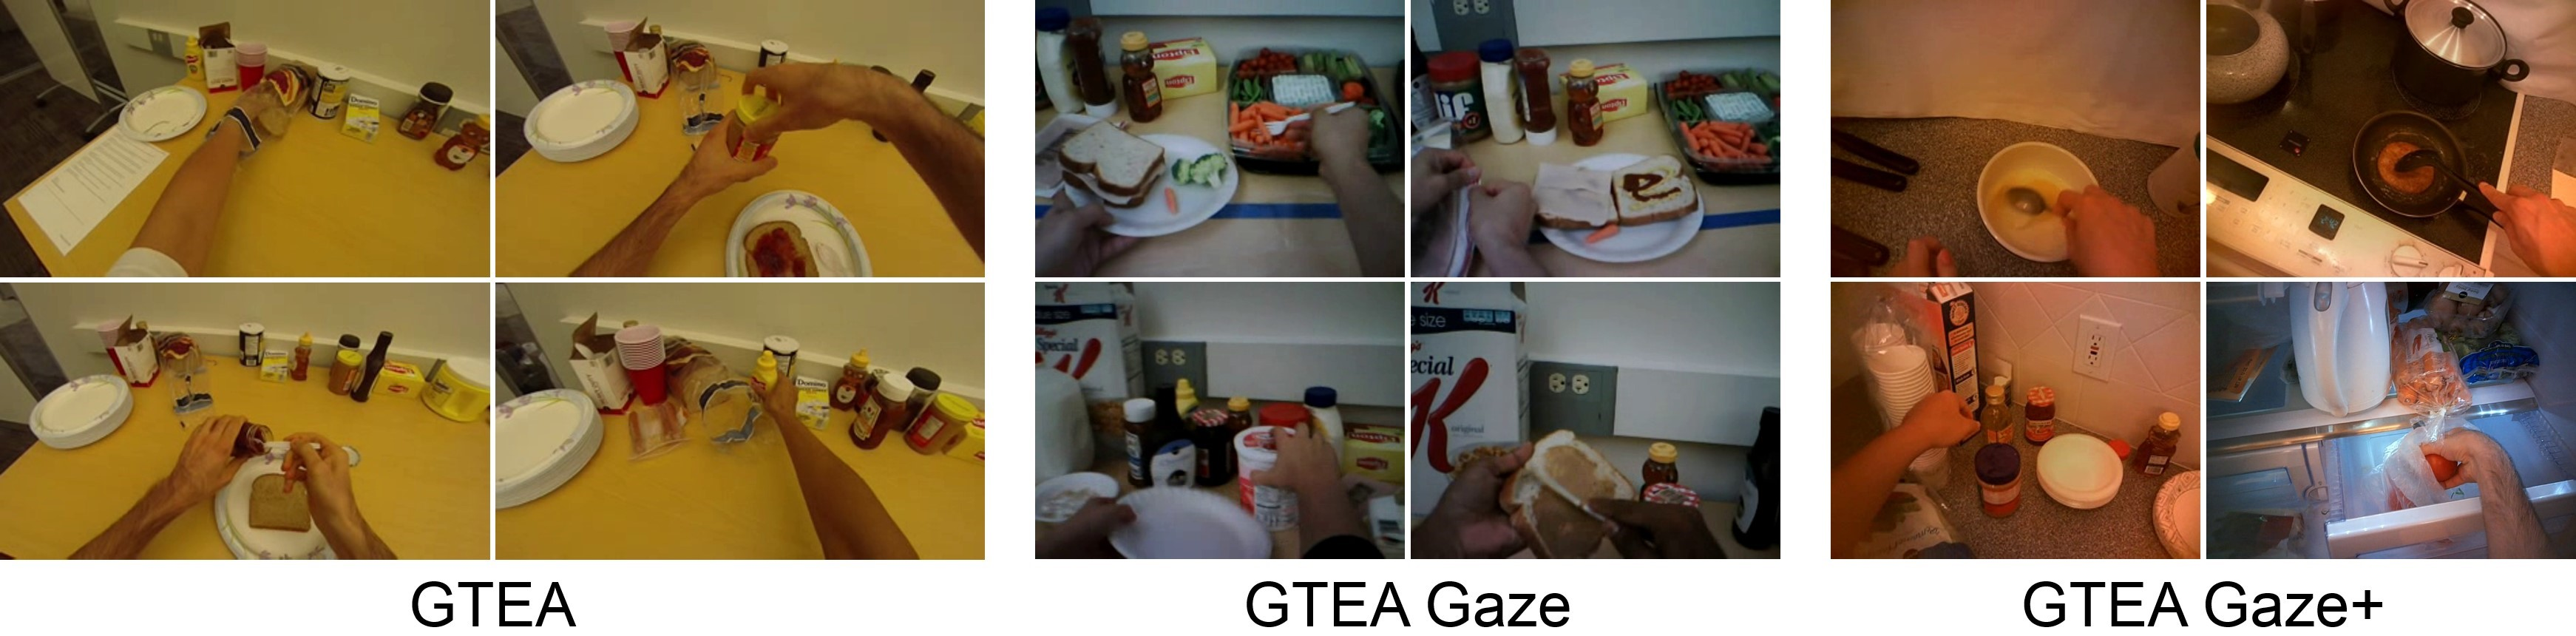
\includegraphics[width=1\linewidth]{Figs/GTEA.jpg}}
%	\caption{Upshots from GTEA family datasets.}
%	\label{fig:gtea}
%\end{figure}
EGTEA Gaze+ \cite{li2020eye} is the largest and most comprehensive dataset for FPV actions and gaze up to date. This dataset coms with HD videos (1920x960), audios, gaze tracking data, frame-level action annotations and pixel-level hand masks at sampled frames. EGTEA Gaze+ is a major expansion of GTEA Gaze+. Specifically, this new datasets EGTEA Gaze + contains 29 hours (withdrawn status) cooking events from 86 independent sessions on 32 topics of 32 subjects performing 7 different meal preparation tasks. These videos have audio and gaze tracking (30Hz). The authors also provide human annotations for actions (human-object interactions) and hand masks. Action annotations include 10325 fine-grained action examples, such as "cut green peppers" or "pour condiments in a condiment container into a salad". These pixel-level hand annotations include 15,176 hand masks in 13,847 frames from the video of 200 action categories sparsely sampled from all 86 sessions of the datasets. Post-processing EGTEA Gaze+ dataset for the thesis’s framework is conducted as follow: The original data in the EGTEA Gaze + dataset is processed into COCO standard in order to be used in the framework. The mask image is converted into binary mask image by thresholding and then applying a contour calculation algorithm of the hand area. At last, the binary mask is converted to the RLE (run length encoding) standard which is usable data in the framework. In the scope of this thesis, the 4 datasets GTEA, GTEA Gaze, GTEA Gaze + and EGTEA Gaze + is regulated into GTEA family datasets.
\vspace*{-\baselineskip}
\begin{figure}
	\centerline{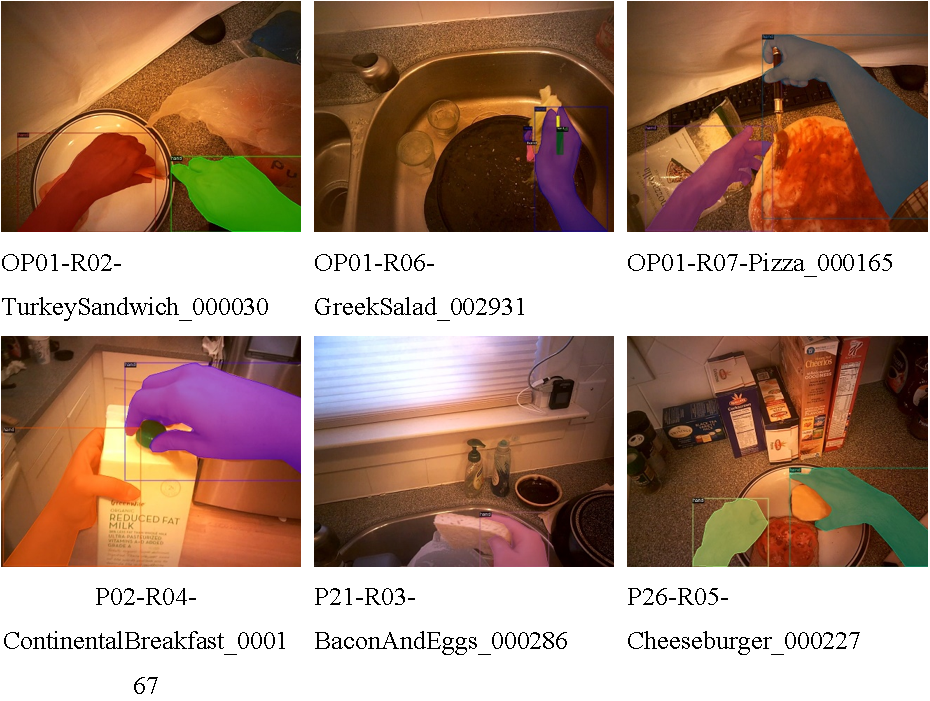
\includegraphics[width=1\linewidth]{Figs/postGTEA.png}}
	\caption{Hand masks after post-processing EGTEA Gaze+.}
	\label{fig:postgtea}
\end{figure}
\subsection{EgoHands dataset}
The EgoHand dataset, which is presented in \cite{10.1109/ICCV.2015.226} is a large dataset for hands in complex egocentric interactions. In order to create as realistic data sets as possible while still being able to carry out some experimental control, the author collected data from different pairs of four pairs of participants, who faced each other when faced with different activities. The authors chose four activities that encourage interaction and gesture movement: (1) playing cards; (2) playing chess, in order to improve efficiency, they encourage participants to focus on speed rather than strategy; (3) solve 24 or 48 pieces of jigsaw puzzles; (4) play Jenga, which involves removing pieces from the 3d puzzle until it collapses. The context is also varied by collecting videos in 3 different locations: a table in a meeting room, a patio table in an outdoor courtyard, and a coffee table at home. The dataset is recorded for several days, and there was no restriction on the clothes of the participants, so there were many types, for example, short-sleeved and long-sleeved shirts, etc. Data is systematically collected from four actors who performed all four activities in all three locations, while randomly assigning participants to interact with each other, resulting in 4 × 4 × 3 = 48 unique video combinations. Each participant wore Google glasses, which recorded a 720 × 1280 video at a frequency of 30 Hz. In post-processing, the videos are synchronized in pairs with each other and each video pair is cut into exactly 90 seconds (2,700 frames). Ground truth is manually annotated from a random subset of 100 frames in each video (approximately one frame per second) using pixel-level manual masks. Each hand pixel has one of the following four tags: the left or right hand of the camera wearer ("my left hand" or "my right hand"), or the left or right hand of the social partner ("your left hand" or "your right hand "). The ground truth was created by six students who were told to mark any hand-shaped pixels they could see, including small hand areas caused by objects being occluded or truncated at frame boundaries. Importantly, compared with EGTEA Gaze+, this dataset defines "hand" as stopping on the wrist, and this job also includes the arm extending toward the participant's sleeve. In total, this dataset contains approximately 130,000 frames of video, of which 4,800 frames have a pixel-level ground truth consisting of 15,053 hands. The partner's hands appear in the vast majority of frames (left and right 95.2\% and 94.0\%, respectively), while the wearer's hand appears less (left and right 53.3\% and 71.1\%, respectively). This may be because one's own hand appears more often outside the camera's field of view, but the right hand appears more frequently because people tend to align their attention with the dominant hand (and all participants are right-handed). Figure \ref{fig:egohands} shows a sample frame with basic facts. This dataset is released on the public web with ground truth accessible through a Matlab API we provided by the authors.
\begin{figure}
	\centerline{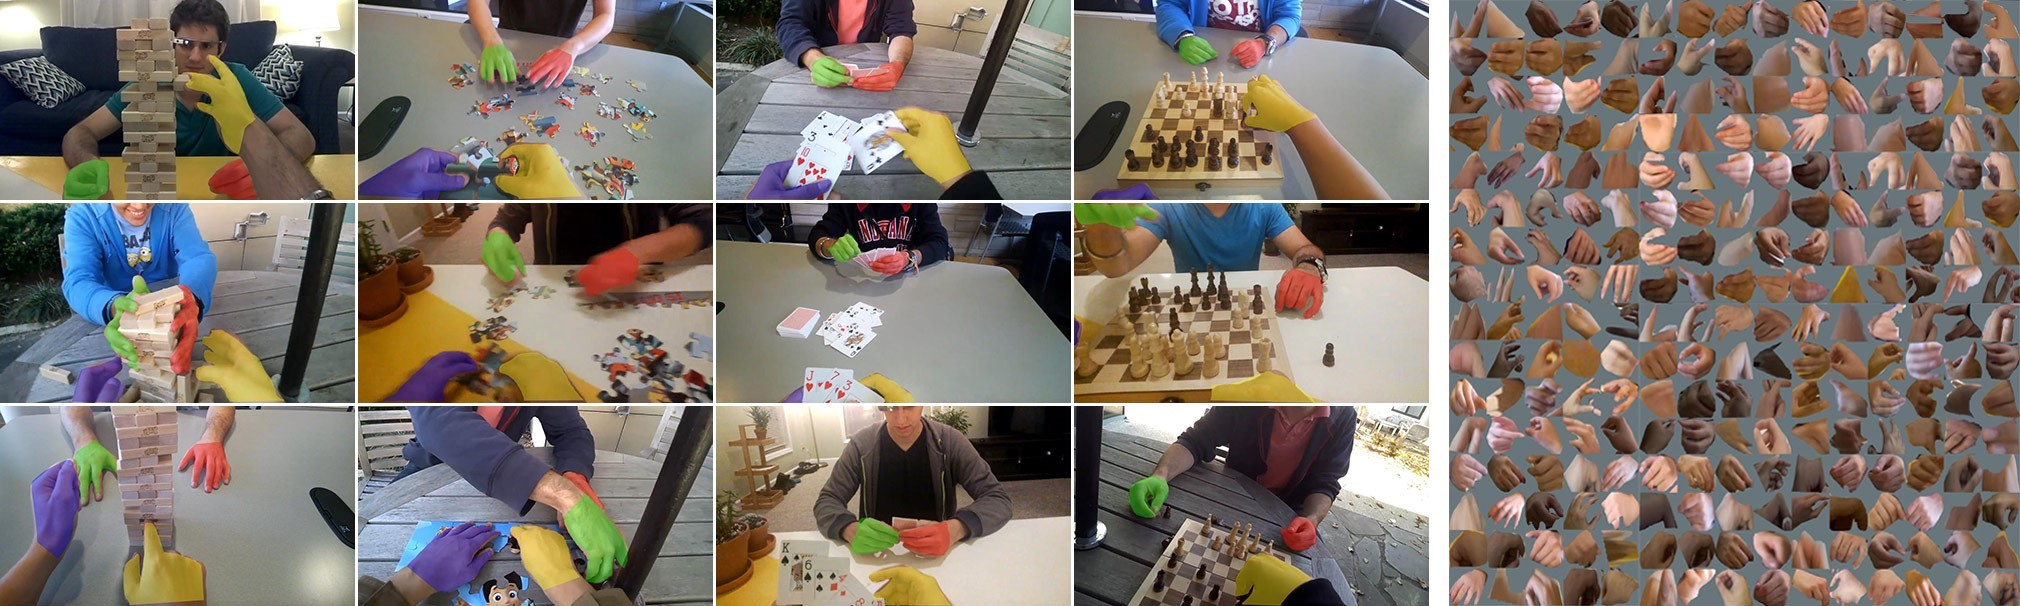
\includegraphics[width=1\linewidth]{Figs/egohands.jpg}}
	\caption{Visualizations of EgoHand dataset in \cite{10.1109/ICCV.2015.226}.}
	\label{fig:egohands}
\end{figure}
Post-processing EgoHands for the thesis’s framework is conducted as follow: The original annotations in EgoHands datasets consists of 4 categories: my left, my right, your left, your right. In the scope of this thesis, I just focus the hands appearing in egocentric video, therefore I convert all 4 categories into 1 category, “hand”. From the “.mat” format data, I dumped into “.json” format and feed to the framework.
%\begin{figure}
%	\centerline{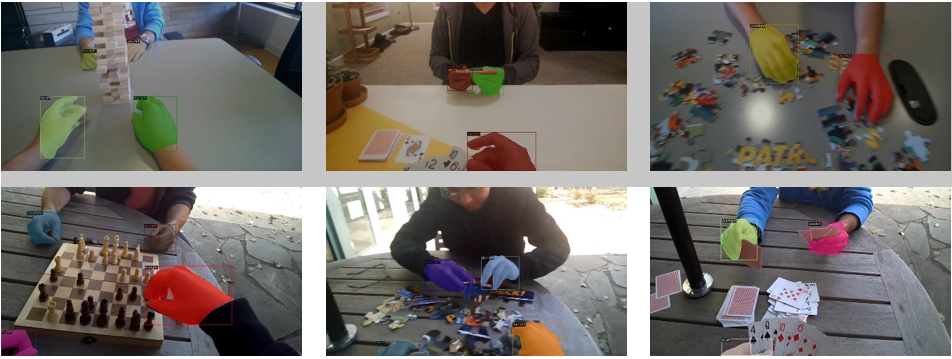
\includegraphics[width=1\linewidth]{Figs/postegohands.png}}
%	\caption{Samples from EgoHands dataset after post-processing.}
%	\label{fig:postegohands}
%\end{figure}
\subsection{Micand32 dataset} \label{subsec:micand32}
As introduced in chapter \ref{chap:intro}, the NAFOSTED’s project is carried out with the aim of using advanced deep learning techniques to evaluate the healing and surgical research of the patient with a sensor through detection segmentation, tracking, gesture recognition, and correlation of the patient's hand with objects. The members in the project prepare the script and perform data collection at Saint Paul Vietnam hospital in one full working week. The experiment was carried out by 10 volunteers, patients aged 20 to 60 years, 5 men and 5 women under the supervision, explanation and help of doctors and instructors. The implementation site consists of 3 areas: the desk area, the sink area and the closet area. Patients will wear 5 sensors including: 1 camera at the head, 1 camera in the shoulder, 1 sensor of kinetics (sensors that will collect and store information about the carrier's position, acceleration) in the left hand, 1 kinematic sensor in the right hand, 1 kinetic sensor in the leg. The patient performs 21 agreed and pre-defined actions, such as taking stairs, practicing hands with objects, brushing hair, opening cabinets, etc. The average number of executions per action is 2. The recorded videos have very high resolution compared to the previous related datasets, is 1920x1440, frequency 30fps. Average time to perform an action is 5 seconds. Thus, in terms of images, the data set consists of 5 people x 2 cameras x 21 actions x 5 times = 1050 videos, so there will be 1050 videos x 5 seconds x 30 fps = 157500 frames.
\\The Micand32 dataset is a subset of the NAFOSTED subject dataset. In the context of the problem of detecting, partitioning and tracking human hands, this thesis is concerned with only 4/21 types of actions most relevant to the hand: (5) practice with ball, (6) practice with water bottles, (7) practice with wooden blocks, (8) practice with cylinders. Figure \ref{fig:micand32} visualizes random samples of 4 action types extracted from MICAND32.
\begin{figure}
	\centerline{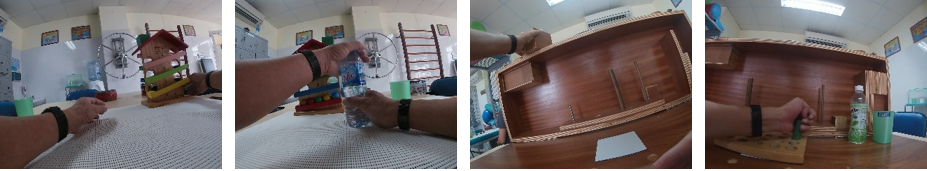
\includegraphics[width=1\linewidth]{Figs/micand32.png}}
	\caption{Randomly selected actions 5 6 7 8, from left to right respectively.}
	\label{fig:micand32}
\end{figure}
Micand32 consists of 32 sequences of 1920x1440 resolution, is divided into 2 parts: Micand32Standard includes 26 sequences and Micand32Enhanced includes 6 sequences. In particular, with Micand32Standard, each sequence contains from 100 to 300 frames, in the frames is mainly the journey of one hand doing a whole activity, this corresponds to the type of short-term tracking. This episode has lengths of each sequences that are equivalent to the MOT Challenge standards. With Micand32Enhanced, each sequence contains from 500 to 1700 frames, of which most frames contain more than 2 arms due to the intervention of the instructor's hand while the patient is performing the action. At the same time, the patient performed multiple repetitions in each sequence, corresponding to a long-term object tracking type. This episode is very close to reality, it is quite challenging and highly applicable. The ground-truth detection and partition section of this data set was labeled by 8 students using the VIA tool \cite{10.1145/3343031.3350535}. VGG Image Annotator is a simple and standalone manual annotation software for images, audio and video. VIA runs in a web browser and does not require any installation or settings. The complete VIA software fits a single independent HTML page, which is less than 400 KB in size and can be run as an offline application in most modern web browsers. The following table \ref{fig:mican32Sta} provides detailed statistics on Micand32.
\begin{table}[]
	\label{fig:mican32Sta}
	\begin{tabular}{|l|l|l|l|l|}
		\hline
		\textbf{No} & Name                         & Action   Type & \begin{tabular}[c]{@{}l@{}}Numbers\\ of frames\end{tabular} & \begin{tabular}[c]{@{}l@{}}Hand/\\ Frame\end{tabular} \\ \hline
		1           & GH010354\_7\_13210\_16534    & 7             & 120                                                         & 1                                                     \\ \hline
		2           & GH010354\_7\_16605\_17602\_1 & 7             & 130                                                         & 1                                                     \\ \hline
		3           & GH010354\_7\_16605\_17602\_2 & 7             & 120                                                         & 1                                                     \\ \hline
		4           & GH010354\_8\_26079\_29031    & 8             & 191                                                         & 1                                                     \\ \hline
		5           & GH010358\_7\_2490\_3390\_1   & 7             & 160                                                         & 1                                                     \\ \hline
		6           & GH010358\_7\_2490\_3390\_2   & 7             & 160                                                         & 1                                                     \\ \hline
		7           & GH010358\_7\_352\_2464\_1    & 7             & 110                                                         & 1                                                     \\ \hline
		8           & GH010358\_7\_352\_2464\_2    & 7             & 135                                                         & 1                                                     \\ \hline
		9           & GH010374\_6\_4944\_6241\_1   & 6             & 140                                                         & 1                                                     \\ \hline
		10          & GH010374\_6\_4944\_6241\_1   & 6             & 100                                                         & 1                                                     \\ \hline
		11          & GH010382\_5\_5725\_7093\_1   & 5             & 100                                                         & 1                                                     \\ \hline
		12          & GH010382\_5\_5725\_7093\_2   & 5             & 130                                                         & 1                                                     \\ \hline
		13          & GH010382\_5\_955\_4771\_1    & 5             & 115                                                         & 1                                                     \\ \hline
		14          & GH010382\_5\_955\_4771\_2    & 5             & 115                                                         & 1                                                     \\ \hline
		15          & GH010382\_6\_18190\_20215\_1 & 6             & 151                                                         & 1                                                     \\ \hline
		16          & GH010382\_6\_18190\_20215\_2 & 6             & 150                                                         & 1                                                     \\ \hline
		17          & GH010382\_6\_20592\_21726\_1 & 6             & 90                                                          & 1                                                     \\ \hline
		18          & GH010382\_6\_20592\_21726\_2 & 6             & 125                                                         & 1                                                     \\ \hline
		19          & GH010382\_8\_16207\_17479\_1 & 8             & 100                                                         & 1                                                     \\ \hline
		20          & GH010382\_8\_16207\_17479\_2 & 8             & 100                                                         & 1                                                     \\ \hline
		21          & GH010383\_5\_462\_968\_1     & 5             & 100                                                         & 1                                                     \\ \hline
		22          & GH010383\_5\_462\_968\_2     & 5             & 120                                                         & 1                                                     \\ \hline
		23          & GH010383\_8\_3221\_3956\_1   & 8             & 100                                                         & 1                                                     \\ \hline
		24          & GH010383\_8\_3221\_3956\_1   & 8             & 100                                                         & 1                                                     \\ \hline
		25          & GH010383\_8\_4544\_5192\_1   & 8             & 100                                                         & 1                                                     \\ \hline
		26          & GH010383\_8\_4544\_5192\_2   & 8             & 100                                                         & 1                                                     \\ \hline
		& MICAND32Standard             & 5, 6, 7,   8  & \textbf{3162}                                               & 1                                                     \\ \hline
		27          & GH010354\_5\_17718\_19366    & 5             & 1684                                                        & 1                                                     \\ \hline
		28          & GH010373\_5\_1284\_2724      & 5             & 1440                                                        & 5                                                     \\ \hline
		29          & GH010358\_6\_10208\_11900    & 6             & 1594                                                        & 4                                                     \\ \hline
		30          & GH010373\_6\_3150\_4744      & 6             & 1692                                                        & 6                                                     \\ \hline
		31          & GH010358\_7\_2490\_3390      & 7             & 900                                                         & 4                                                     \\ \hline
		32          & GH010358\_8\_8000\_8547      & 8             & 547                                                         & 3                                                     \\ \hline
		& MICAND32Enhanced             & 5, 6, 7,   8  & \textbf{7857}                                               & 4                                                     \\ \hline
		& MICAND32                     & 5, 6, 7,   8  & \textbf{11019}                                              & 2                                                     \\ \hline
	\end{tabular}
\caption{Detailed enumeration of the Micand32 dataset.}
\end{table}
In order to evaluate the effectiveness of the tracking algorithm, there is currently no standard popular tool to support the id tag of the object in the video frame. To the best of my knowledge, currently there is no egocentric dataset that involves detailed standard for hand tracking, according to \cite{9064606}. This thesis refers to the MOT Challenge tracking data standard and the annotator has done the tracking tagging through a self-developed tool called EHTA. Egocentric Hand Tracking Annotator was especially designed to model semi-automatic annotation pipelines to speed up the annotation process. Such a semi-automatic can be achieved by using AI generated annotation proposals that are presented to an annotator inside the annotation tool. Also, EHTA integrates a part of the VIA labeling tool \cite{10.1145/3343031.3350535}.
Figure \ref{fig:micand32Trajectory} performs trajectory of the patient’s hands opening water bottle, in which the groundtruth is visualized by EHTA.
\begin{figure}
	\centerline{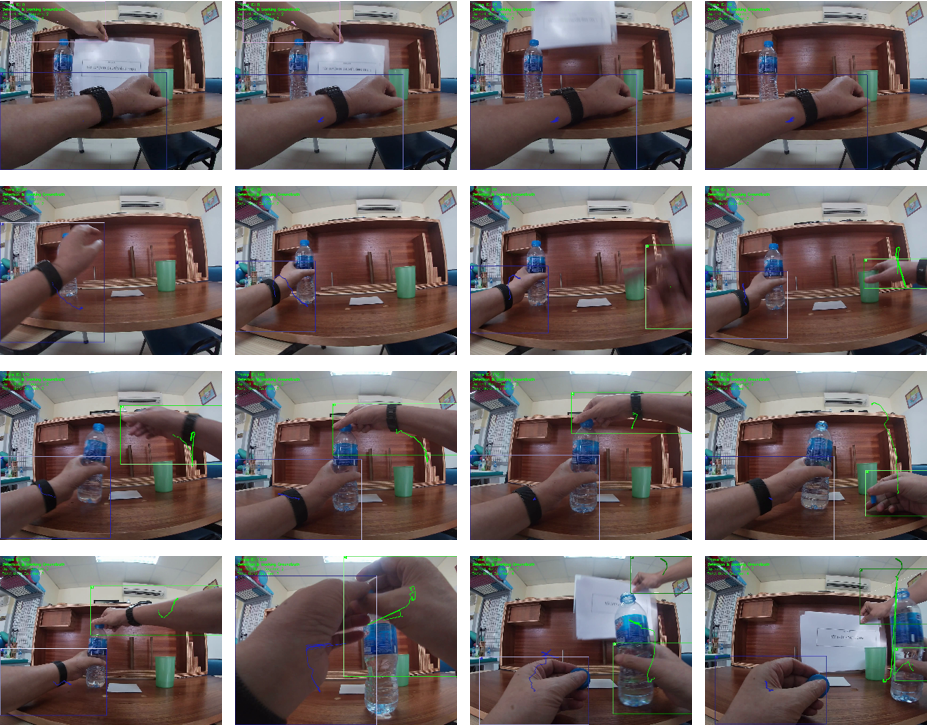
\includegraphics[width=1\linewidth]{Figs/micand32Trajectory.png}}
	\caption{Visualization of groundtruth tracklets of patient’s hands opening water bottle. Series of continuous samples from video GH010358\_6\_10208\_11900 in Micand32Enhanced.}
	\label{fig:micand32Trajectory}
\end{figure}
Figure \ref{fig:EHTA} shows the working flowchart of EHTA. Initially, annotator selected 1 model from model zoo that was pre-trained on COCO, GTEA family and EgoHands datasets, for example, this thesis used FasterRCNNR50FPN3x. Input is a set of frames in 1 sequence. For each frame, reference the model on the frame to predict the position of the hands and get the detection of bounding box and confidence score. Next, use the VIA tool to display the prediction in frames, observe and make comments to write code. From observation and experience with the dataset, writing code to automatically editing the labels for the hand’s position and identification. Then shows the automatically assigned label portion. If the label is not correct, manually correct the bounding box position, add or remove the bounding box, or correct the incorrect ID. Finally, save ground-truth according to MOT Challenge standards for training, testing and evaluation in txt format. At the same time, save ground-truth video for debugging.
\begin{figure}
	\centerline{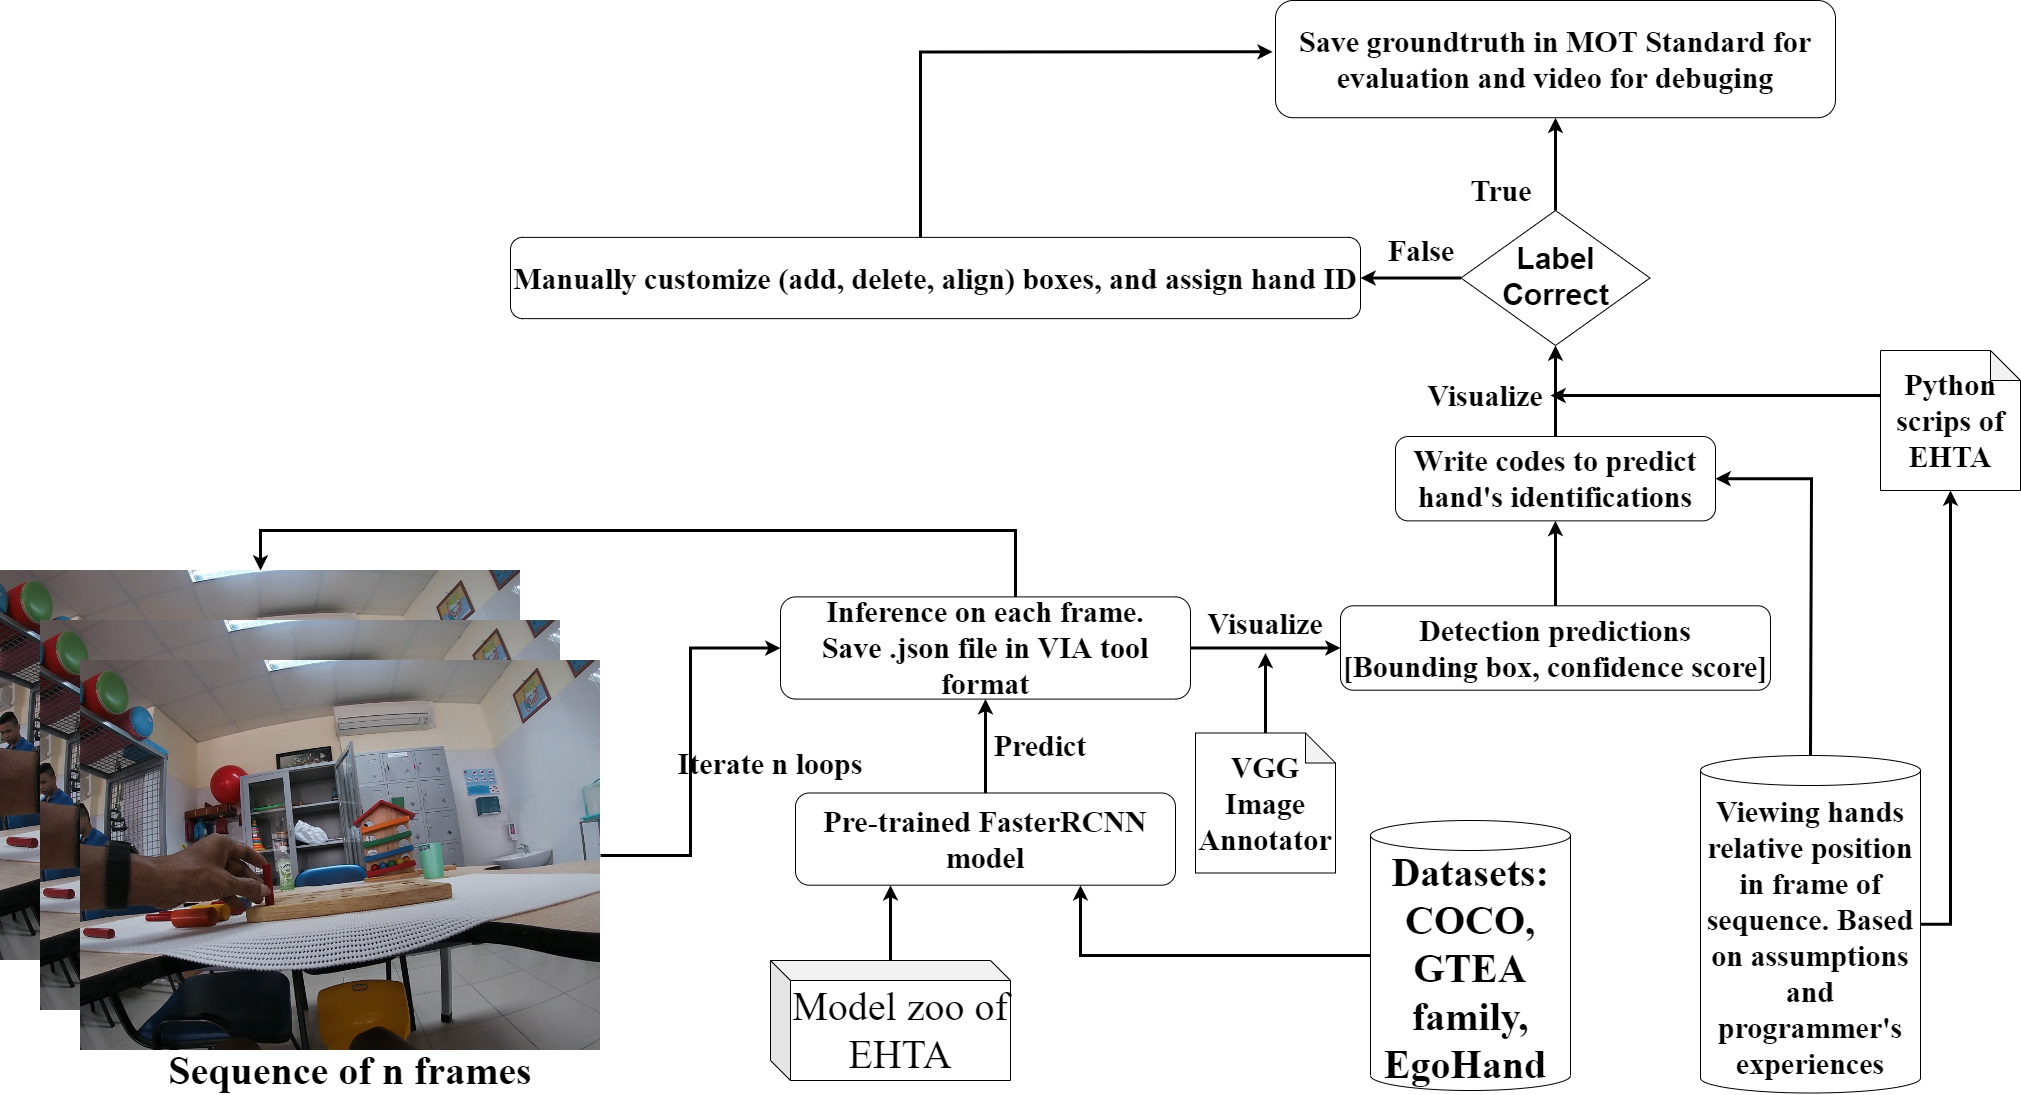
\includegraphics[width=1\linewidth]{Figs/EHTAflowchartPage2.png}}
	\caption{The workflow of EHTA.}
	\label{fig:EHTA}
\end{figure}
Annotation time for 1 image with manually and semi-automatically by EHTA is respectively 5 seconds and 1 second. By using EHTA, the subjectivity of human perception and loss of time are reduced as well as consistency and coordination among different individuals' annotations are accomplished.